This section will analyse the market of the preliminary idea. It will go into detail with potential competitors, the customer segment, the positioning of the product and the pricing of the product.

\subsection{Competitors}
Competitors in the market needs to be identified, in order to position the application in the market.

Within the region where the application is planned to be implemented, there are few competitors that rent out fishing equipment. 

Fiskekurser.dk is based in Svendborg, in the south of Funen. Their primary business focuses on fishing courses, but it is also a possibility to rent equipment and go fishing by yourself.
The prices are difficult to find on their website, and it seems you have to call them to find out.
When contacting Fiskekurser.dk, they said that they try to rent out equipment to private fishers, but they had bigger success, with just focusing on fishing courses and excursions. This might be due to the fact, that it is difficult to find any products or rental pricing on their page.
Several other businesses and one put-and-take, were called and approximately half of them had equipment, which they either lent or rented to customers.

\subsection{Customer Segment}
\begin{figure*}[t!]
  \centering
  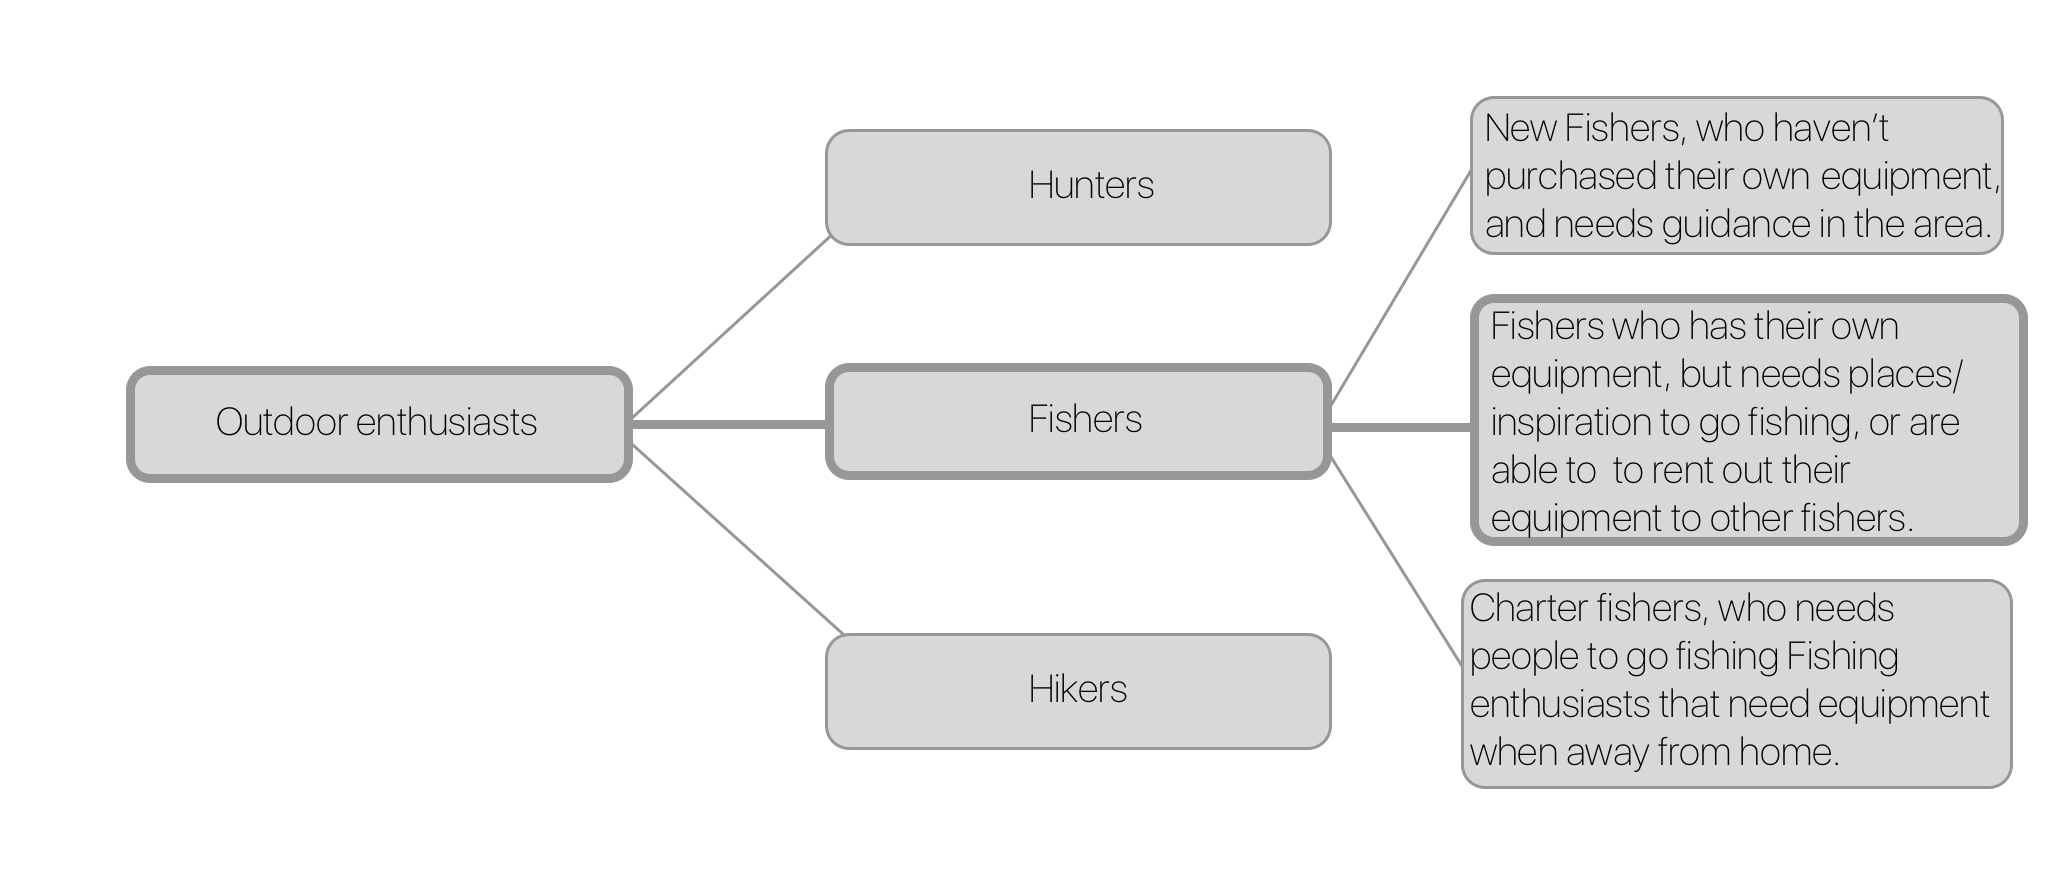
\includegraphics[width=0.7\textwidth]{images/SegmentTree}
  \caption{Customer Segment Tree}
\end{figure*}



The overall customer segment  which the product is intended for, is outdoor enthusiasts. Out of that category, there are three sub categories, Fishers, Hikers and Hunters. From these sub categories the Fisher-category has been selected, as it has a great potential in gaining a lot of users. The Fisher-category can further be divided into three groups, as seen in the mind map. The prioritised customer segment, was chosen to be: The fishers that need equipment, when away from home.  

Another segment, which has been discussed, is the businesses, which could gain value from use of the platform. Examples of such businesses, range from outdoor shops to Businesses, who take people on fishing trips, and private people who rents their own spare equipment out for a price.

\subsection{Positioning}
The application should to be different from other similar products. The application delivers several different niches, for the fishing universe, in one product. That's why the product is different from others, because it is intended to give the users easy access, to everything they need for fishing, in just one application. The advantage is, that the application is the first, which is offering this kind of service. This means that the application doesn't have any direct competitor. Those who are offering similar services for fishing right now, aren't competitors, actually they are a part of the idea, since the application can also be beneficial for them.



\subsection{Pricing}
The team has decided upon using the freemium business model, see \autoref{sec:businessModel} for further information.

The business application will require a business subscription. The fee of a business subscription will be 550 DKK/month or 6600 DKK/year.

The business application is meant for commercial users, and will contain a range of features, which can help the businesses grow.



\subsection{Market Survey}
To investigate the market and customer segment further, an electronic Google forms survey was distributed via Facebook to fishing enthusiast pages, and through our own networks on facebook. 97 individuals responded to the survey. The following section will discuss the data obtained from the survey. 


94.6\% of our respondents are male respondents. This is in line with a report published in march 2010 by the Danish Ministry of Food, Agriculture and Fishing. The information could be used for marketing, to add more masculine values into the campaign.


77.2\% of the respondents answered that they have equipment for more than one person. This is a lot of people, but this might be because a lot of the respondents came from sport fishing groups on Facebook.


22.8\% were interested in renting out their equipment and 26\% were interested in renting equipment from others. Even though this number seems small, it is actually huge (if this is to be interpreted as representative, which it probably isn’t), as the number of fishers world-wide is an enormous number, and 22.8\% of them is a significant share.


60.8\% of the respondents fished outside their own region and in other countries.


Only 10.6\% of our respondents have had bad experiences, when renting equipment.


57.9\% of the respondents has had difficulties in establishing contact with locals, to rent/loan a boat to fish from. The platform could be a possible solution for this, as it allows boat owners to rent out their boats for fishing purposes.


The survey might have been biased, as we have distributed it via. sport fishing groups on facebook, and the respondents from these groups aren’t exactly in the target customer segment, so this was a bad decision, for this kind of survey.
This might have caused some numbers to become different than the numbers the group anticipated.


When asked why the respondents hadn’t rented equipment, it became clear that the respondents were from a more enthusiastic group of fishers. 59.7\% said that they always have had their own equipment, 23.6\% said they hadn’t tried to rent. From this it can be concluded, that there should have been made a more general survey, which was directed more at the wanted customer segment.


In the survey, the respondents were asked if they have had any problems with bringing their own equipment to a fishing trip in a foreign country. The group anticipated that the answers would indicate, that it was a problem to bring their own equipment. But it was in fact the opposite.
When the answers was investigated further, it showed that there was a tendency that the people who had no problem with bringing their own equipment, were fishing only in scandinavia and northern europe. And the few respondents who agreed that it could be problematic, were fishing overseas.
From this, the group interpreted that it is not a problem to bring your own equipment for destinations, not that far from home. It becomes a problem, the further away you have to travel.


The user survey has helped the group to identify new features, which can add value for the users. It also increased the team's knowledge of the users.


\subsection{Interview with Possible Advertisers}
Seven phone calls were made, of which three were to physical shops, three were to online shops and one for a put and take lake. The physical shops were found on Krak.dk and the online shops on Google.
All of them were using various kinds of advertisement. Among those were Google AdWords, Facebook, E-banners, Radio advertising, newspapers and magazines.


Half of them were willing to share information, about how much they were spending on advertisement.

The put and take lake was the only one who used radio advertising, which costs roughly 11.000 DKK for a 20 sec. spot, that airs 10 times per day, during a week (Kilde: Radio Skala - Fyn). The online shop “fiskegrej.dk” was using about 40.000 DKK on different types of advertisement pr. month, which is properly why they were found at the top of the list on Google. This is a bias, since we did not get to talk with the average online shop.
It is now known that the big shops are willing to spend 10.000 DKK pr week on advertising. The owner of fiskegrej.dk, said that he would spend about 1000-3000 DKK to advertise on an application.

Upon this it can be conclude, that the estimated average price of 550 DKK. pr. month to advertise through the application, is realistic. This is concluded since fiskegrej.dk is one of the companies that allready spend a lot on advertisings, and other smaller companies probely don´t and won´t spent that much.
The price to advertise on the application depends on how much you want to be seen, just like Google AdWords, and the price will therefore be individual.\footnote{Link to interview (Danish): \url{https://docs.google.com/document/d/1ncEAEWFtBWFb4BxMuvz63bWnEAdJT_po1jBjIvsiWco/edit?usp=sharing}}  
